
\documentclass [a4paper,12pt]{paper}

\usepackage{mycommands}
\title{Lecture 16: Ray theory}
\author{David Al-Attar \\ Michaelmas Term, \the\year}


\begin{document}

\maketitle

\section*{Outline and Motivation}

In the previous lecture we examined the propagation of plane elastic waves. Here we consider what happens when the material 
parameters are not constant, 
developing a ray theory that provides a \textbf{good approximation in situations when the length-scale of the 
heterogeneity is large relative to that of the waves}. Essentially, the waves always look locally 
planar, but as they propagate the wavefronts gradually deform, and the amplitudes can be changed by focusing 
and defocusing effects. This ray theory is related to elastodynamics in the same manner that 
geometric optics is related to Maxwell's equations, with both being "high frequency" approximations in a 
suitable sense. There are also close links with what is known as semi-classical analysis, this 
being the subject in which the behaviour of quantum mechanical systems are studied in the "classical limit" $\hbar\rightarrow0$.

\section*{Relative length scales of heterogeneity}

We consider the linearised motion of an elastic body occupying a whole space whose material parameters are 
constant everywhere except a bounded region in which $\rho$ and $A_{ijkl}$ can vary smoothly. 
For definiteness, let $p_{i}^{0}$ be the slowness vector of elastic waves within the homogeneous part of the body, and 
assume that the heterogeneous region is contained within the half-plane $p_{i}^{0}x_{i}\ge0$. 
Within the homogeneous half plane $p_{i}^{0}x_{i}<0$ we know that plane wave solutions are possible of the form
\begin{equation}
u_{i}(x,t)=f(t-p_{i}^{0}x_{i})a_{i}^{0}
\end{equation}
and our aim is to extend this solution suitably into the heterogeneous region. In general there exists no exact
closed-form solution  to this problem, and so it must be studied either through numerical calculations 
or using approximate methods. While numerical calculations are of huge practical value, they provide 
relatively little physical insight, and so we shall focus on physically motivated approximate methods.


\begin{figure}[ht]
\centering
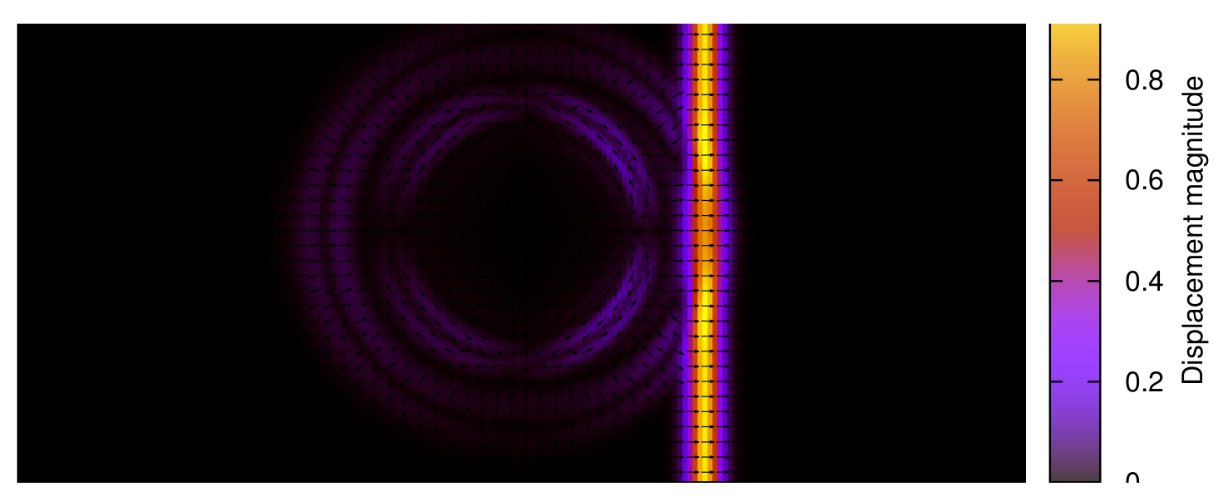
\includegraphics[width=0.8\textwidth]{figures/L5F1.png}
\caption{Scattering of a plane p-wave in a homogeneous background model due to its inter-
action with a heterogeneity having a typical length-scale approximately equal to
the length-scale of the incident wave. The arrows show the particle motion, and
we see that the scattered wave field is comprised of both P-waves and S-waves.}
\label{fig:fig1}
\end{figure}

In broad terms there are three possible approaches for studying this problem, with the appropriate choice being determined
by the relative length scales of the incident wave and the heterogeneous structure. Let $\lambda$ 
denote the \textbf{dominant wavelength for the plane wave}, and denote by $L$ the \textbf{smallest length scale over which 
the material parameters vary to an appreciable extent}. If their ratio satisfies
\begin{equation}
\frac{L}{\lambda}\approx1
\end{equation}
then we expect the incident wave to be \textbf{scattered by the heterogeneity}. There is not sufficient time in this course to 
discuss scattering of seismic waves further, though it is an important physical process within the Earth, 
and can be analysed using the \textbf{Born approximation} that you may know from quantum mechanics. 

In this lecture we shall focus on situations when
\begin{equation}
\frac{L}{\lambda}\gg1
\end{equation}
which is to say the length scale of the heterogeneity is much greater than the length scale of the incident wave. Here we 
do not expect to see significant scattering of the incident wave, but instead a smooth evolution of the 
wavefront as it propagates through the heterogeneity, along with associated amplitude variations due to focusing effects. This 
is the domain of \textbf{geometric ray theory}.


Finally, we might ask what happens in the case that
\begin{equation}
\frac{L}{\lambda}\ll1
\end{equation}
This is actually very applicable to the Earth, as rocks are made up of small grains of different minerals that can have 
quite distinct physical properties, and yet observed seismic waves have wavelengths on the order of kilometres 
to thousands of kilometres. We also lack the time to enter into this topic in any detail, but it can be shown 
that such waves ``see'' a suitably averaged version of the body that appears smooth on the length scale of the incident waves.
The appropriate smoothed medium can be determined using the methods of \textbf{homogenisation theory}. Again, there
is sadly not time within this course to discuss this topic further.


\begin{figure}[ht]
\centering
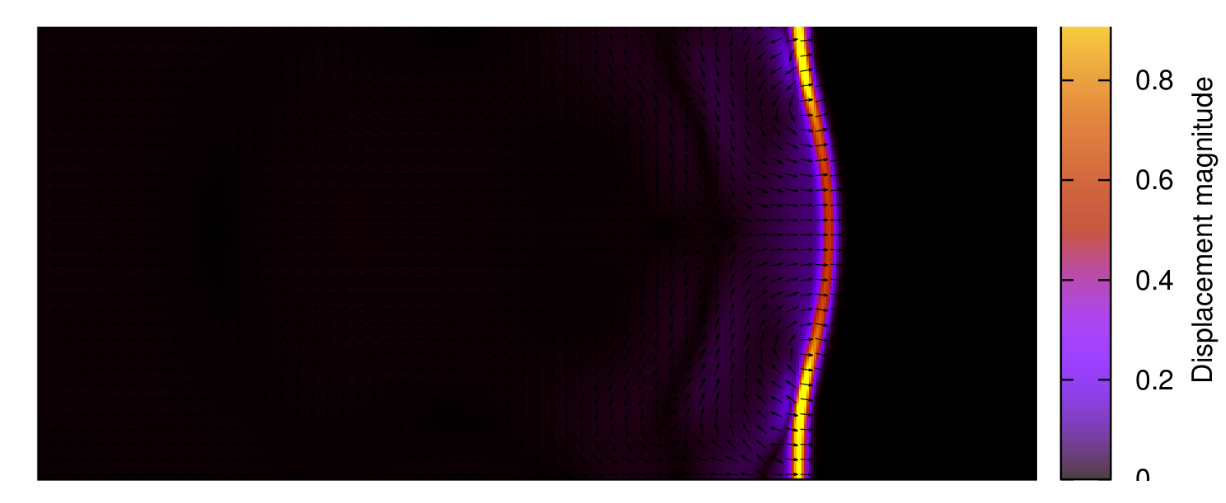
\includegraphics[width=0.8\textwidth]{figures/L5F2.png}
\caption{Passage of a plane p-wave through a heterogeneous region having length-scale much
larger than that of the incident wave. Here we see minimal scattering, along with
the smooth distortion of the wave front and associated amplitude and polarisation
variations. This is a situation to which ray theory can be usefully applied.}
\label{fig:fig2}
\end{figure}

\section*{The ray series ansatz}

As noted above, we shall focus on situations where the length scale of the heterogeneity is long 
relative to the length scale of the incident plane wave. As a first guess, we might expect that the continuation of 
the plane wave into the heterogeneous region can be approximated in the following manner
\begin{equation}
u_{i}(x,t)=f[t-T(x)]a_{i}(x)
\end{equation}
with this expression taking account of the following physical ideas:
\begin{enumerate}
    \item The linear phase term $t-p_{i}^{0}x_{i}$ has been replaced with the non-linear term $t-T(x)$. This allows the 
    wavefronts in the heterogeneous region to curve as they propagates through regions with different wave speeds;
    \item The amplitude and polarisation term $a_{i}^{0}$ has been replaced with a function of position $a_{i}(x)$ which 
    allows for (i) focusing and defocusing effects during propagation and (ii) changes in the particle motion associated 
    with both wavefront curvature and variations in anisotropic properties.
\end{enumerate}
We will call the function $T$ the \textbf{travel time}, and note that the wavefronts of eq.(5) are, by definition level surfaces
\begin{equation}
T(x)=\text{constant}.
\end{equation}
It will be useful to define the \textbf{local slowness vector} in terms of this travel time by setting
\begin{equation}
p_{i}=\frac{\partial T}{\partial x_{i}}
\end{equation}
which is everywhere orthogonal to the wavefronts. Note that the local slowness vector is equal 
to the slowness vector within homogeneous regions where the travel time depends linearly on $\mathbf{p}$.

To proceed, it is useful to decompose displacement vector fields into an integral 
over harmonic plane waves
\begin{equation}
u_{i}(x,t)=\frac{1}{2\pi}\int_{\mathbb{R}}\tilde{f}(\omega)e^{\ii[t-T(x)]}a_{i}(x)\dd\omega,
\end{equation}
It is clear that eq.(5) is the temporal convolution of the singular plane wave
\begin{equation}
u_{i}(x,t)=\delta[t-T(x)]a_{i}(x)
\end{equation}
with the waveform f. In what follows, it will be convenient to focus on such singular waves, and from now on 
we set $\tilde{f}(\omega)=1$ or equivalently $f(t)=\delta(t)$.

We could try to use the ansatz in eq.(9) as a 
starting point for the development of ray theory, but experience has shown that it is necessary to consider 
instead the following generalisation
\begin{equation}
u_{i}(x,t)=\frac{1}{2\pi}\int_{\mathbb{R}}\sum_{n=0}^{\infty}\frac{a_{i}^{n}(x)}{(\ii\omega)^{n}}e^{\ii\omega[t-T(x)]}\dd\omega,
\end{equation}
where we note that the $n$ in $a_{i}^{n}$ is a superscript and not an exponent. This expression is known as the \textbf{elastodynamic 
ray series}. The $n=0$ term within this expression is equivalent to the eq.(9). The physical meaning or need for the additional terms 
within the expansion is less clear, and indeed, these terms are typically ignored within practical applications. But 
as an initial comment, we note that each successive term within the series is divided by a factor of $1/(\ii\omega)$, and within the Fourier domain 
this is equivalent to a temporal integration. Thus the terms within this series are getting progressively smoother and smoother.

\subsection*{Substitution into the equations of motion}
We recall that the linearised equations of motion for an elastic body can be written
\begin{equation}
\rho\frac{\partial^{2}u_{i}}{\partial t^{2}}-\frac{\partial}{\partial x_{j}}\left(A_{ijkl}\frac{\partial u_{k}}{\partial x_{l}}\right)=0,
\end{equation}
where we are not here allowing a body force associated with a seismic source. Within the temporal Fourier domain this equation becomes
\begin{equation}
-\omega^{2}\rho u_{i}-\frac{\partial}{\partial x_{j}}\left(A_{ijkl}\frac{\partial u_{k}}{\partial x_{l}}\right)=0
\end{equation}
where for simplicity we use the same symbol for the displacement vector and its Fourier transform. From eq.(10) we see that the 
ray series in the Fourier domain is simply
\begin{equation}
u_{i}(x,\omega)=\sum_{n=0}^{\infty}\frac{a_{i}^{n}(x)}{(\ii\omega)^{n}}e^{-\ii\omega T(x)}.
\end{equation}
From eq.(7) and eq.(13) we find that
\begin{align}
\frac{\partial u_{k}}{\partial x_{l}}&=\sum_{n=0}^{\infty}\frac{1}{(\ii\omega)^{n}}\left(\frac{\partial a_{k}^{n}}{\partial x_{l}}
-\ii\omega p_{l}a_{k}^{n}\right)e^{-\ii\omega T}, \\
A_{ijkl}\frac{\partial u_{k}}{\partial x_{l}}&=\sum_{n=0}^{\infty}\frac{1}{(\ii\omega)^{n}}A_{ijkl}\left(\frac{\partial a_{k}^{n}}
{\partial x_{l}}-\ii\omega p_{l}a_{k}^{n}\right)e^{-\ii\omega T}.
\end{align}
Taking the divergence of the second expression, we  obtain
\begin{multline}
\frac{\partial}{\partial x_{j}}\left(A_{ijkl}\frac{\partial u_{k}}{\partial x_{l}}\right)=\sum_{n=0}^{\infty}\frac{1}
{(\ii\omega)^{n}}\left[\frac{\partial}{\partial x_{j}}\left(A_{ijkl}\frac{\partial a_{k}^{n}}{\partial x_{l}}\right)
-\ii\omega\frac{\partial}{\partial x_{j}}(A_{ijkl}p_{l}a_{k}^{n}) \right. \\
\left. -\ii\omega A_{ijkl}p_{j}\frac{\partial a_{k}^{n}}{\partial x_{l}}+(\ii\omega)^{2}A_{ijkl}p_{j}p_{l}a_{k}^{n}\right]e^{-\ii\omega T}.
\end{multline}
and substituting into the frequency domain equations of motion in eq.(12) we arrive at
\begin{multline}
\sum_{n=0}^{\infty}\frac{1}{(\ii\omega)^{n}}\left[\frac{\partial}{\partial x_{j}}\left(A_{ijkl}\frac{\partial a_{k}^{n}}{\partial x_{l}}\right)-\ii\omega\frac{\partial}{\partial x_{j}}(A_{ijkl}p_{l}a_{k}^{n}) \right. \\
\left. -\ii\omega A_{ijkl}p_{j}\frac{\partial a_{k}^{n}}{\partial x_{l}}+(\ii\omega)^{2}A_{ijkl}p_{j}p_{l}a_{k}^{n}-(\ii\omega)^{2}\rho a_{i}^{n}\right]e^{-\ii\omega T}=0 .
\end{multline}

The above equation must hold for all frequencies, and this can only be true if the coefficient of each power of $\ii\omega$ is separately equal to zero. From the coefficients of the highest-order term $(\ii\omega)^{2}$ we obtain
\begin{equation}
[A_{ijkl}p_{j}p_{l}-\rho\delta_{ik}]a_{k}^{0}=0,
\end{equation}
while those for the $\ii\omega$ term take the form
\begin{equation}
[A_{ijkl}p_{j}p_{l}-\rho\delta_{ik}]a_{k}^{1}=\frac{\partial}{\partial x_{j}}(A_{ijkl}p_{l}a_{k}^{0})+A_{ijkl}p_{j}\frac{\partial a_{k}^{0}}{\partial x_{l}},
\end{equation}
and then for a general term with $n\ge2$
\begin{equation}
[A_{ijkl}p_{j}p_{l}-\rho\delta_{ik}]a_{k}^{n}=\frac{\partial}{\partial x_{j}}(A_{ijkl}p_{l}a_{k}^{n-1})+A_{ijkl}p_{j}\frac{\partial a_{k}^{n-1}}{\partial x_{l}}-\frac{\partial}{\partial x_{j}}(A_{ijkl}\frac{\partial a_{k}^{n-2}}{\partial x_{l}})
\end{equation}
The first of these equations depends on only the local slowness vector and the zeroth-order polarisation vector. We will see shortly that 
this equation can be solved for the travel time $T$ and also gives the orientation of $a^{0}(x)$ at each point. 
Having done this, solution of eq.(19) gives the amplitude of the zeroth-order term, while eq.(20) can be used to successively 
determine the higher-order polarisation vectors. We will not, however, discuss the solution of these higher-order equations
 within this course.

At this stage it is reasonable to ask where exactly we have made an approximation? Assuming that the above set of equations 
can be solved for $T$ and all the $a^{n}$ then it would seem that we have obtained an exact solution to the equations of motion. 
For this to be a valid conclusion, however, we must then think carefully about the sense in which the ray series converges. 
Though we will not enter into this topic in detail, the key point is \textbf{the ray series  is  not convergent in any usual sense}. 
Indeed, the problem is at low frequencies, with the series being very badly behaved at $\omega=0$. To force this series to converge, 
we could zero-out the solution in some neighbourhood of $\omega=0$, but by doing this we would be left with  an approximate 
solution to the equations of motion. Because, however, the error lies only within a bounded range of frequencies it must be a smooth 
function. Building on such ideas, it can be shown that the ray theoretic solution \textbf{exactly predicts the 
 singular part of the wavefield}, but that there is a \textbf{smooth error term whose size need not be small}\footnote{These ideas are
formalised within the theory of \textbf{Fourier integral operators} developed in the 1970s by Lars Hormander and others.}.

\section*{The eikonal equation}

Within this section, we show that eq.(18) can be solved for the travel time $T$ using the so-called \textbf{method of characteristics}. 
This is a useful method that can be applied to both linear and non-linear first-order partial differential equations, 
and reduces their solution to the integration of systems of ordinary differential equations. In fact, it is through 
solution of these ordinary differential equations that rays will enter into the theory in a natural manner.

Before  applying this technique,  we must first reduce eq.(18) into a single partial differential equation for the travel time. 
To do this, it will be useful to define the \textbf{local Christoffel operator} through
\begin{equation}
\Gamma_{ik}(x,\mathbf{p})=\frac{1}{\rho(\mathbf{x})}A_{ijkl}(\mathbf{x})p_{j}p_{l}.
\end{equation}
for all $x\in\mathbb{R}^{3}$ and vectors $\mathbf{a}$ and $\mathbf{p}$. We can then write eq.(18) in the form
\begin{equation}
\{\bm{\Gamma}[\mathbf{x},\mathbf{p}(\mathbf{x})]-\mathbf{I}\}\mathbf{a}^{0}(\mathbf{x})=\mathbf{0},
\end{equation}
which closely resembles the Christoffel equation we encountered in the study of elastic plane waves. Indeed, 
the physical intuition underlying ray theory is that locally the solutions behave like plane waves.
 At each point, $\mathbf{x}$, we know that eq.(22) may be satisfied by a non-trivial polarisation vector 
 $\mathbf{a}^{0}(\mathbf{x})$ if and only if the local slowness vector $\mathbf{p}(\mathbf{x})$ is a solution of
\begin{equation}
\det\{\bm{\Gamma}[\mathbf{x},\mathbf{p}(\mathbf{x})]-\mathbf{I}\}=0,
\end{equation}
which is known in the context of ray theory as an \textbf{eikonal equation}. Eq.(23) can be interpreted as requiring
 that at each $\mathbf{x}$, the local slowness vector $\mathbf{p}(\mathbf{x})$ lies on the \textbf{local slowness surface}.


Having determined the appropriate local slowness vector $\mathbf{p}(\mathbf{x})$, eq.(22) then implies that $\mathbf{a}^{0}(\mathbf{x})$ lies 
within the eigenspace of $\bm{\Gamma}[\mathbf{x},\hat{\mathbf{p}}(\mathbf{x})]$ with eigenvalue equal to the square of the corresponding 
local phase speed. For simplicity, we shall only consider materials whose local slowness surfaces are everywhere non-degenerate, and so we can write
\begin{equation}
\mathbf{a}^{0}(\mathbf{x})=A_{0}(\mathbf{x})\hat{\mathbf{a}}^{0}(\mathbf{x}),
\end{equation}
where $A_{0}(\mathbf{x})$ a scalar amplitude, and $\hat{\mathbf{a}}^{0}(\mathbf{x})$ is the appropriate normalised eigenvector  which is 
determined uniquely up to its sign. We have assumed that the local slowness surfaces within the body are everywhere non-degenerate, 
and can therefore, always write the eikonal equation unambiguously in the form
\begin{equation}
\{||\mathbf{p}(\mathbf{x})||^{2}c_{1}[\mathbf{x},\hat{\mathbf{p}}(\mathbf{x})]^{2}-1\}\{||\mathbf{p}(\mathbf{x})||^{2}c_{2}[\mathbf{x},\hat{\mathbf{p}}(\mathbf{x})]^{2}-1\}\{||p(\mathbf{x})||^{2}c_{3}[\mathbf{x},\hat{\mathbf{p}}(\mathbf{x})]^{2}-1\}=0
\end{equation}
where $c_{k}(\mathbf{x},\hat{\mathbf{p}})$ denotes the local phase speed at $\mathbf{x}$ corresponding to the $k$th sheet and with 
propagation direction $\hat{\mathbf{p}}$. At an initial point only one of these factors will vanish, say the $k$th one,
and by continuity it is the same factor that vanishes elsewhere. As a result, the eikonal equation is reduced to the simpler form
\begin{equation}
||\mathbf{p}(\mathbf{x})||^{2}c_{k}[\mathbf{x},\hat{\mathbf{p}}(\mathbf{x})]^{2}-1=0
\end{equation}
and this is the equation we will aim to solve.

\subsection*{The method of characteristics}
To solve the reduced form of the eikonal equation we will proceed in a way that will likely seem rather unmotivated. We 
introduce the \textbf{ray Hamiltonian} for the $k$th sheet of the local slowness surface
\begin{equation}
H_{k}(\mathbf{x},\mathbf{p})=\frac{1}{2}||\mathbf{p}(\mathbf{x})||^{2}c_{k}[\mathbf{x},\hat{\mathbf{p}}(\mathbf{x})]^{2},
\end{equation}
which is defined on a six-dimensional \textbf{phase space} comprised of points $(\mathbf{x}, \mathbf{p})$, and allows us 
to write the eikonal equation eq.(26) in the alternate form
\begin{equation}
H_{k}[\mathbf{x},\mathbf{p}(\mathbf{x})]=\frac{1}{2}, \quad \mathbf{p}(\mathbf{x})=(\nabla T)(\mathbf{x}).
\end{equation}
Eq.(28) states that the desired solution, $T$, of the eikonal equation corresponds to a \textbf{three-dimensional level surfaces}
 $H_{k}(\mathbf{x},\mathbf{p})=\frac{1}{2}$ of the ray Hamiltonian. This 
geometric viewpoint is central to the method of characteristics. 

The \textbf{initial data} we have for the problem  is that  on the plane
\begin{equation}
p_{i}^{0}x_{i}=0, 
\end{equation}
the travel time is constant, and we are free to set this value equal to zero. We then wish to continue this solution into 
the heterogeneous region $p_{i}^{0}x_{i}\ge0$. 
Each point $\mathbf{x}^{0}$ on this initial plane corresponds to a point $(\mathbf{x}^{0},\mathbf{p}^{0})$ within the phase space, 
and at such points eq.(28) is satisfied.
In this manner, the initial data for the problem specifies a \textbf{two-dimensional level surface $S^{0}$ of the ray Hamiltonian}, and to 
solve the eikonal equation, we must construct
 a three-dimensional level surface $S$ containing $S^{0}$.

Let $(\mathbf{x}^{0},\mathbf{p}^{0})$ be a point on the initial plane $S^{0}$, and consider the solution of 
\textbf{Hamilton's canonical equations} for the ray Hamiltonian $H_{k}$ as defined by
\begin{equation}
\frac{\ddns x_{i}}{d\sigma}=\frac{\partial H_{k}}{\partial p_{i}}, \quad \frac{\ddns p_{i}}{d\sigma}=-\frac{\partial H_{k}}{\partial x_{i}}
\end{equation}
subject to the initial conditions
\begin{equation}
x_{i}(0)=x_{i}^{0}, \quad p_{i}(0)=p_{i}^{0}.
\end{equation}
Within these equations, $\sigma$ is a \textbf{generating parameter} whose physical interpretation will become clear but 
initially is just a parameterisation for the resulting integral curves.
A key property of Hamilton's equations is that the \textbf{Hamiltonian is conserved along their solutions}. Indeed, using the chain rule we obtain
\begin{equation}
\frac{\ddns}{\ddns\sigma}H[\mathbf{x}(\sigma), \mathbf{p}(\sigma)]=\frac{\partial H}{\partial x_{i}}\frac{\ddns x_{i}}{\ddns\sigma}+\frac{\partial H}{\partial p_{i}}\frac{\ddns p_{i}}{d\sigma} = -\frac{\ddns p_{i}}{d\sigma}\frac{\ddns x_{i}}{\ddns\sigma}+\frac{\ddns x_{i}}{d\sigma}\frac{\ddns p_{i}}{\ddns\sigma}=0,
\end{equation}
where on the right hand side we have suppressed arguments for clarity. As we have $H_{k}(\mathbf{x}^{0},\mathbf{p}^{0})=\frac{1}{2}$ each point
 on the initial surface, it follows that $H_{k}[\mathbf{x}(\sigma), \mathbf{p}(\sigma)]=\frac{1}{2}$ along the 
curve within phase space obtained by integration of eq.(30) subject to the given initial conditions. What we can then do is take in 
turn each point $(\mathbf{x}^{0},\mathbf{p}^{0})$ of the initial plane, and integrate Hamilton's equations to produce a 
curve on which the ray Hamiltonian is equal to one half. The union of all these curves defines a smooth three-dimensional 
surface within the phase space, and this gives us the desired solution of the eikonal equation in geometric form. 

In detail, this 
solution is usually defined only locally near to $S^{0}$, and we shall return to this point in a moment. Furthermore, it is not 
actually clear that such level surfaces need to be formed from the graph of $\nabla T$ for some travel time function $T$. 
Indeed, through this process, we obtain a value for $\mathbf{p}$ for each $\mathbf{x}$, and hence a vector field 
$\mathbf{p}(\mathbf{x})$. But this vector field is meant to be the gradient of a scalar function, and hence  
its first derivatives must possess the non-trivial symmetry
\begin{equation}
    \frac{\partial p_{i}}{\partial x_{j}}=\frac{\partial p_{j}}{\partial x_{i}}.
\end{equation}
Using the method's of \textbf{symplectic geometry} -- a beautiful subject that is intrinsically linked to Hamilton's equations -- 
it can be shown that the necessary symmetry of $\mathbf{p}(\mathbf{x})$ does hold, and hence a valid travel time is locally 
defined. 


\begin{figure}[ht]
\centering
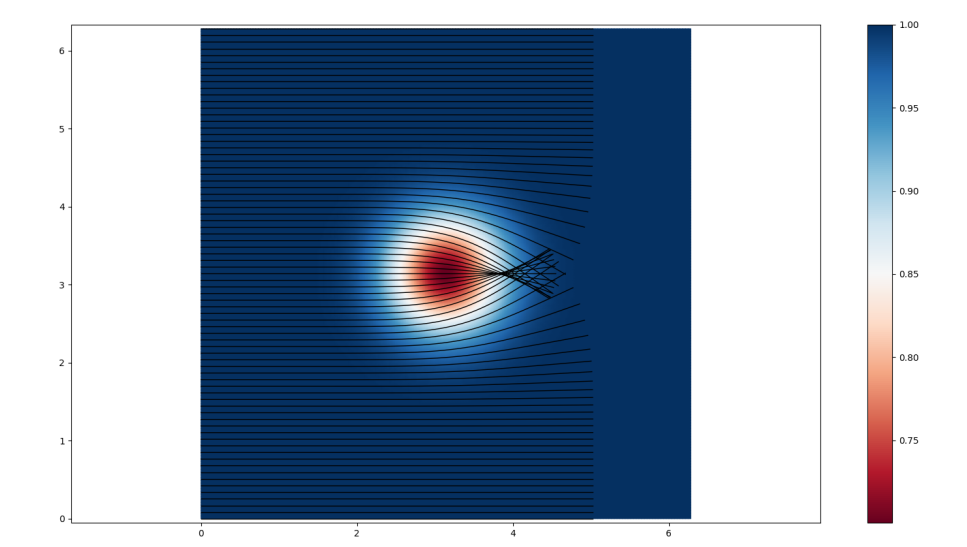
\includegraphics[width=0.8\textwidth]{figures/L5F3.png}
\caption{An example of ray tracing within a heterogeneous body, and of the formation of a
caustic due to an area of low velocity.}
\label{fig:fig3}
\end{figure}

Having constructed the level surface $S$, how do we recover the travel time $T$? We first make use of eq.(7) and (30) to obtain
\begin{equation}
\frac{\ddns}{\ddns\sigma}T[\mathbf{x}(\sigma)]=\frac{\partial T}{\partial x_{i}}\frac{\ddns x_{i}}{\ddns \sigma}=p_{i}\frac{\partial H}{\partial p_{i}}
\end{equation}
To simplify the result, we note that the ray Hamiltonian $H_{k}(\mathbf{x},\mathbf{p})$ is a homogeneous function of $\mathbf{p}$ of 
degree two, meaning
\begin{equation}
H_{k}(\mathbf{x},\gamma \mathbf{p})=\gamma^{2}H_{k}(\mathbf{x},\mathbf{p}),
\end{equation}
for all real $\gamma$. Euler's homogeneous function theorem\footnote{
    You do not need to know this theorem. In isotropic media the necessary calculation can be performed explicitly, 
    and this is the only case you might be asked to reproduce this derivation.} then implies
\begin{equation}
p_{i}\frac{\partial H}{\partial p_{i}}=2H_{k},
\end{equation}
and from eq.(28) we conclude that
\begin{equation}
\frac{\ddns }{\ddns \sigma}T[\mathbf{x}(\sigma)]=1.
\end{equation}
On the initial surface $S^{0}$ the travel time is everywhere equal to zero, and so eq.(36) has the trivial solution
\begin{equation}
T[\mathbf{x}(\sigma)]=\sigma
\end{equation}
along the curve starting from each initial point $(\mathbf{x}^{0},\mathbf{p}^{0})$. In this manner, we can 
identify the generating parameter with the travel time along an integral curve. 

The curves $\sigma\mapsto \mathbf{x}(\sigma)$ formed by projection of solutions of Hamilton's equations in phase space onto the
position variable are known as \textbf{rays}. In order for the travel time $T$ constructed by the above method 
to be a \textbf{single-valued function} of $\mathbf{x}$, then it is necessary that each point $\mathbf{x}$ within the heterogeneous 
region is joined to a point $\mathbf{x}^{0}$ on the initial plane by a \textbf{unique ray}. Indeed, if there were two such 
rays, then for each we could calculate a travel-time through the above method, and there is no reason why these two times 
should be equal. 

Points $\mathbf{x}$ within the heterogeneous region that can be reached by rays starting at two or 
more points on the initial plane are called \textbf{caustics}, and at such points ray theory breaks down. Though we do not have 
time to look quantitatively at the the behaviour of the scalar amplitude $A^{0}(\mathbf{x})$ introduced in eq.(24), 
it can be shown that this ray theoretical amplitude becomes \textbf{infinite at caustics}. In reality, caustics are characterised by 
large but finite amplitudes (the name comes from the Latin for ``to burn''), and more 
sophisticated asymptotic techniques  allow them to be handled quantitatively.

Though within this lecture, we have focused on a problem of an initially plane wave entering into a heterogeneous region, it should
 be apparent that ray theory can be applied to problems having more general initial conditions. For example, the initial data for the 
 travel time can be specified on  a curve or even at a point. Furthermore, it is possible to extend the method to allow for discontinuities
in material parameters along internal boundaries so long as they are smooth relative to the wavelength of the waves considered.

\section*{What you need to know and be able to do}
\begin{itemize}
    \item[(i)] The form of the ray-series expansion, and understand its underlying physical motivation.
    \item[(ii)] How to obtain the eikonal equation and transport equations by substituting the ray expansion into the equations of motion. The full derivation given in the lecture is too involved to occur within an exam, but you may be asked to apply these methods within simpler situations.
    \item[(iii)] Understand how the eikonal equation can be interpreted geometrically within a six-dimensional phase space, and be able to explain how solutions can be obtained through integration of Hamilton's equations.
    \item[(iv)] Be able to solve the Hamiltonian ray equations in simple cases, and also to deduce some of their properties. Practice in this will be given in the next lecture and within the final example sheet.
    \item[(v)] What a caustic is, and why ray theory breaks down there.
\end{itemize}




\end{document}


